\begin{figure}%[b]
    	\centering
    	\begin{minipage}{0.3\textwidth}
    		\centering
    		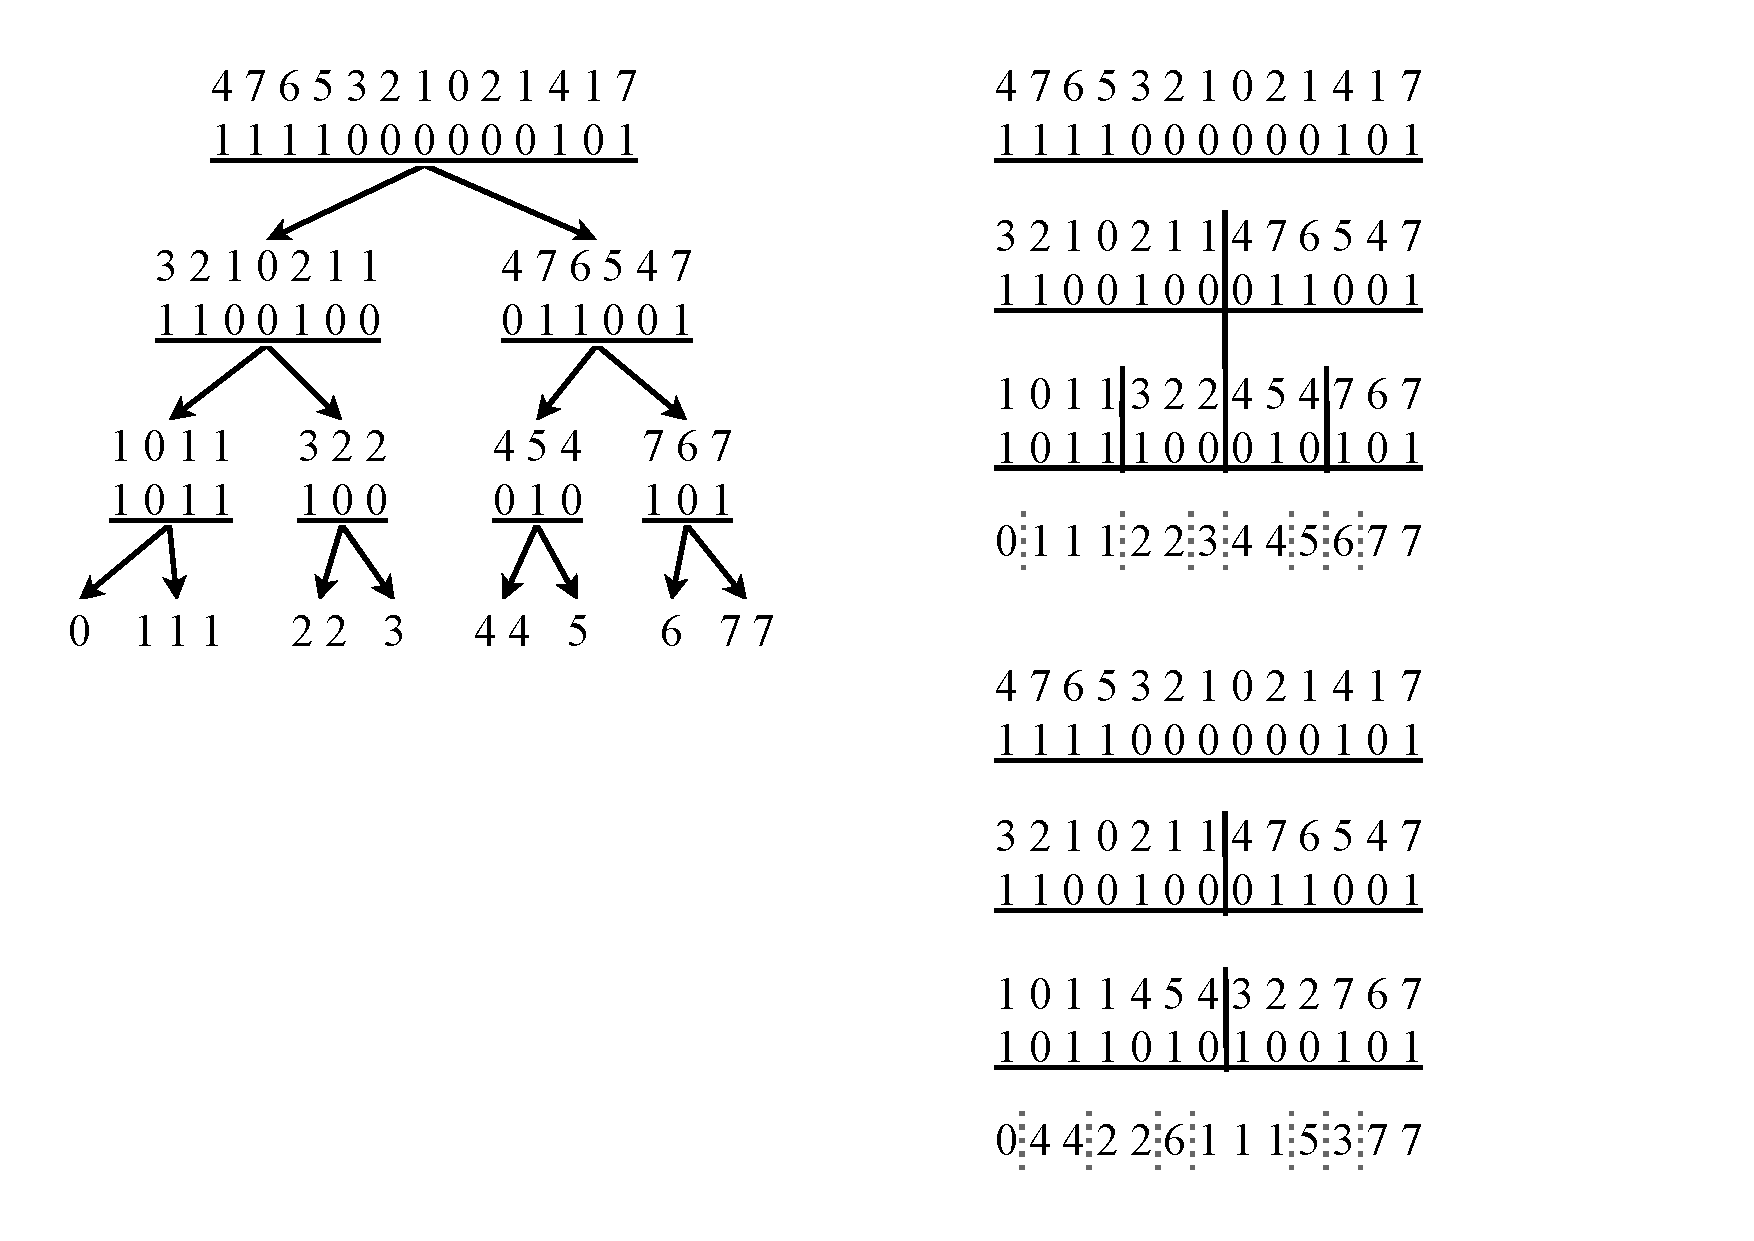
\includegraphics[scale=.4, clip,  trim=30 280 440 30]{img/arte/graphs-wavelet-matrix.pdf}
    		
    		(a)
    	\end{minipage}
    	\begin{minipage}{0.3\textwidth}
    		\centering
    		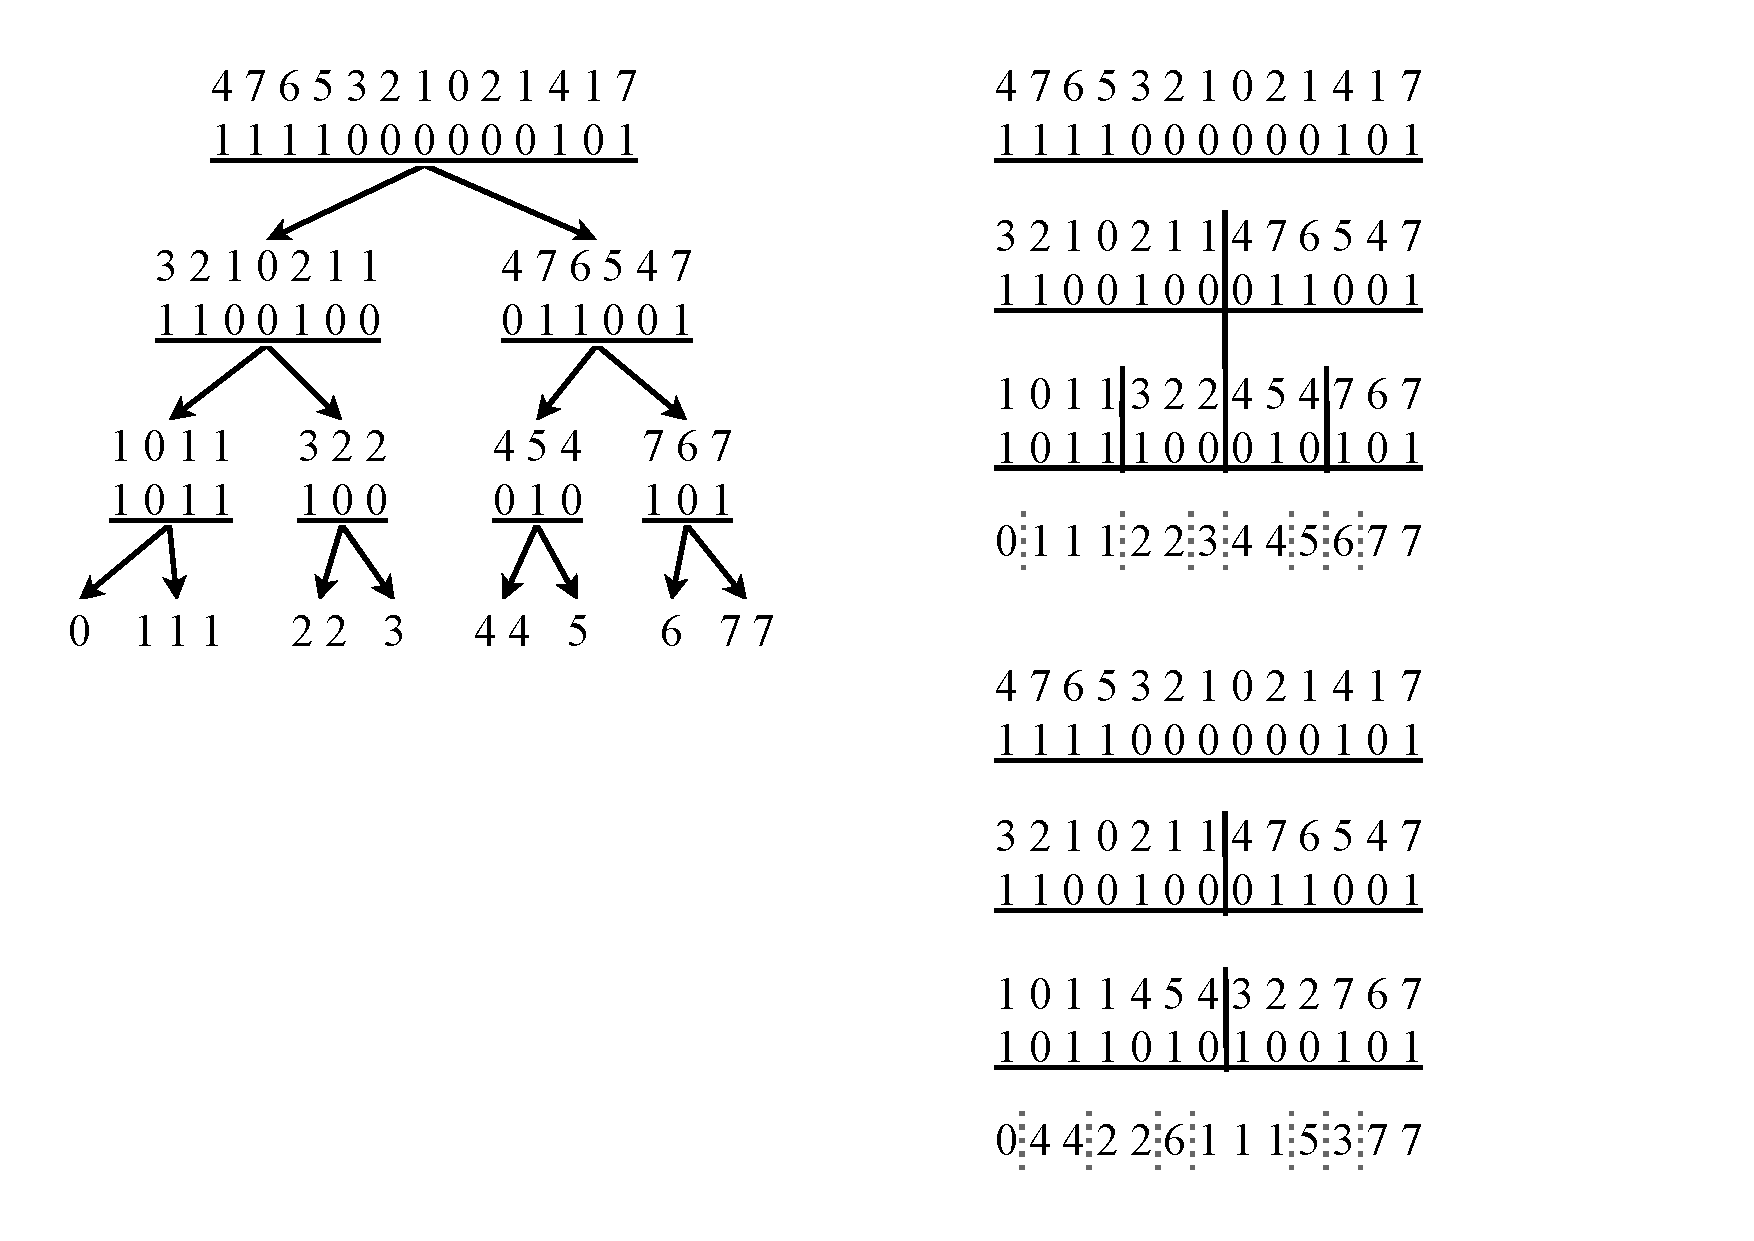
\includegraphics[scale=.45, clip, trim=470 320 170 30]{img/arte/graphs-wavelet-matrix.pdf}

    		(b)
    	\end{minipage}
    	\begin{minipage}{0.3\textwidth}
    		\centering
    		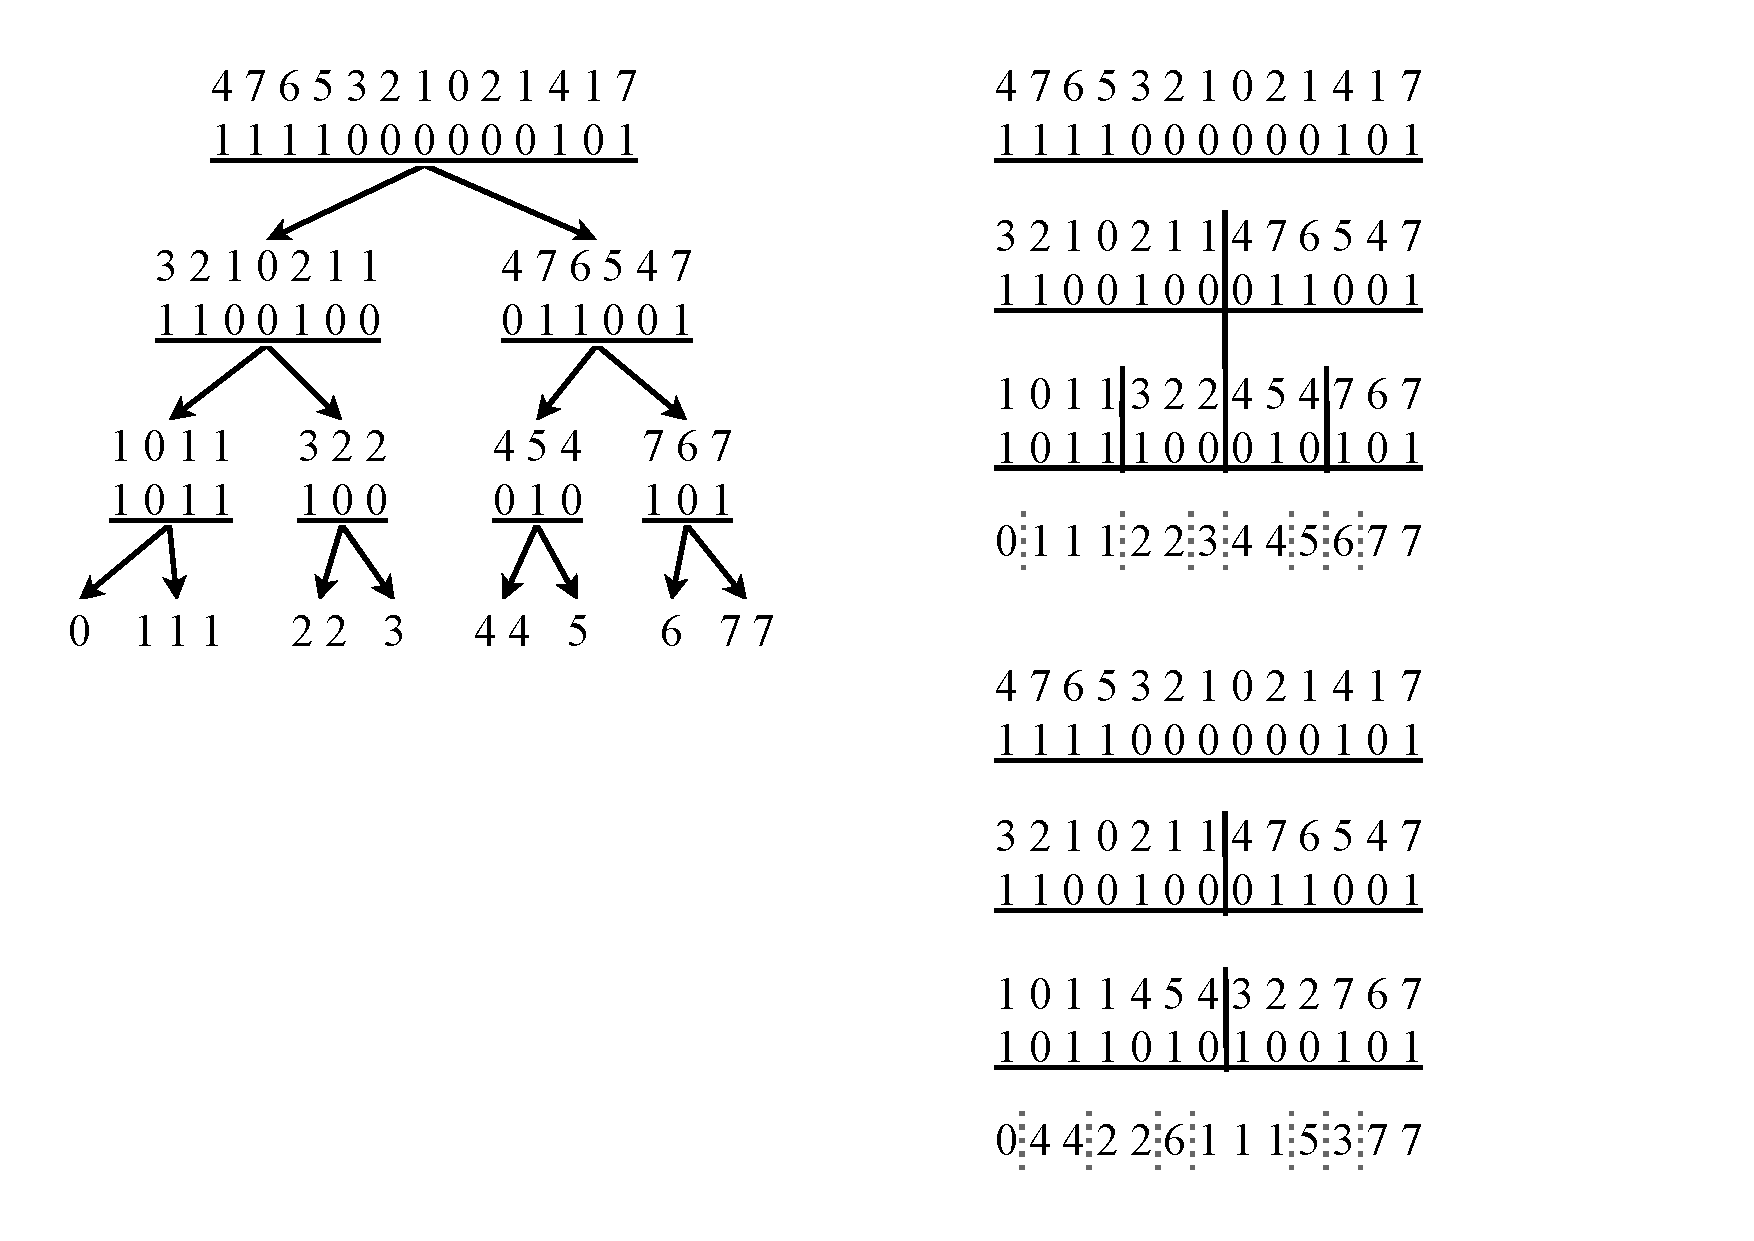
\includegraphics[scale=.45, clip, trim=470 33 170 317]{img/arte/graphs-wavelet-matrix.pdf}

    		(c)
    	\end{minipage}

    \caption{Ejemplos para wavelet-matrix. (a) Un wavelet tree. (b) El mismo wavelet tree sin punteros. (c) La wavelet matrix correpondiente.}
    \label{fig:wavelet-matrix}
\end{figure}
